\documentclass[a4paper]{article}
\usepackage{anysize}
\marginsize{1cm}{1cm}{1cm}{1cm}

\usepackage{amssymb}
\usepackage{amsmath}
\usepackage{graphicx}
\usepackage{epsfig}
\usepackage{subfigure}
\usepackage{listings}
\usepackage{natbib}
\usepackage{verbatim}
\usepackage[T1]{fontenc} 
\lstset{language=haskell}
\lstset{commentstyle=\textit}
\lstset{mathescape=true}
\lstset{backgroundcolor=,rulecolor=}
\lstset{basicstyle=\ttfamily}
%\linespread{2.0}

\begin{document}

\title{\bf Monadic Reference Counting}

\author{Giuseppe Maggiore \quad
		  Michele Bugliesi
 \\ Universit\`a Ca' Foscari Venezia
 \\ Dipartimento di Informatica 
 \\ \{maggiore,bugliesi\}@dsi.unive.it
}

\date{}
\maketitle

\begin{abstract}
In this paper we show how a powerful memory and resource management technique such as reference counting can be implemented transparently as a library through the use of monads. While this is interesting in itself, since garbage collectors are not always the best choice for all programs, our paper also shows how the bind and return operators can be used to correctly identify the lifetime of resources and references. Finally, we discuss how with a powerful enough type system and the use of a parameterized monad we can track various interesting properties about the state of stateful computations. In our case we track the set of resource-types that the program handles, but we argue that in other cases this technique could be used to track even more complex and interesting properties.
\end{abstract}

\section{Introduction}
\label{sec:intro}
%%%%%%%%%%%%%%%%%%%%%%%%%%%%%%%%%%%%%%%%%%%%%%%%%%%%%%%%%%
% intro.tex
%%%%%%%%%%%%%%%%%%%%%%%%%%%%%%%%%%%%%%%%%%%%%%%%%%%%%%%%%%

Game are:
- complex
- require performance

Low-level languages do not cut it fully.

We will:
(A) discuss game constraints
  - discuss traditional approaches and their limitations
  - discuss similarities between game genres and try and find a general framework
  - define a language that is built around this general framework, and which makes it easy
  - reason on why we'd rather have a new language and not just a library
  - give syntax, typing, semantics
(B) give optimization transformations of the language
(C) give a detailed case study
  - give benchmarks that show how effective our optimizations are and how they are completely automated (they require no effort on the part of the programmer) 

\section{State Monad}
\label{sec:state_monad}
%----------------------------------------------------------------------------
%  state_monad.tex 
%----------------------------------------------------------------------------
The state monad \cite{1_1,1_2,1_3,1_4,1_5} is a monad which allows us to write stateful, imperative computations in a pure language without sacrificing purity. A value of state monad type represents a statement, and its type requires that a value of type \emph{state} is passed as a parameter to the statement in order for it to evaluate to its result. Evaluating a statement not only returns the result of the evaluation, but also the new value of the state: the input state may have been modified, that is the evaluation of any statement may produce side-effects.

The type of the state monad reminds the type of the denotational semantics of an imperative statement. This is interesting, in that we could consider values of the state monad as the denotation of statements:

\begin{lstlisting}
type St s a = s -> (a,s)
\end{lstlisting}

We can bind statements together into composite statements and return values inside statements. When binding, we concatenate the two statements by evaluating the first and then plugging its result into the second and then evaluating it:

\begin{lstlisting}
(>>=) :: St s a -> (a -> St s b) -> St s b
p >>= k = \s ->
  let y,s' = p s
  in k y s'
\end{lstlisting}

When we wish to pack a value x inside a monad we return it:

\begin{lstlisting}
return :: a -> St s a
return x = \s -> x,s
\end{lstlisting}
 

\section{Reference}
\label{sec:reference}
%----------------------------------------------------------------------------
%  reference.tex 
%----------------------------------------------------------------------------
The state monad as presented above is well-known and commonly used in pure languages such as Haskell. This kind of world- passing-style (or store-passing-style) is powerful and allows a programmer to write perfectly fine imperative code. Since this monad is mostly (if not always exclusively) used to pass around the state and manipulate mutable portions of the state through the use of references and proxies, we now propose an extension of the monad that focuses exclusively on these references.
A system resource is anything that we wish to release as soon as we are done with it. System resources may include streams, network connections, GPU memory in GPGPU applications (as done, for example, in \cite{9_1,9_2}), threads, etc. In some cases even memory references may be treated as resources, especially when we wish to recycle memory as soon as possible rather than just leave the job to the garbage collector. A system resource can be defined in terms of an appropriate type class:

\begin{lstlisting}
class Reference f a s where
  new :: a -> St s (f a)
  incr :: f a -> St s ()
  decr :: f a -> St s ()
  get :: f a -> St s a
  count :: f a -> St s Int
\end{lstlisting}

A Reference is represented by a functor f and a type a. a is the type of our actual resource, and f a is the proxy that we will use to access this resource. The proxy f a may:
\begin{itemize}
\item be created from a value a with new
\item increment its internal counter with incr
\item decrement its internal counter with decr
\item get its internal value with get
\item get its internal counter with count
\end{itemize}

The only public functions that we leave accessible are new and get. The other functions can only be called from inside the monad implementation.

\subsection{Reference axioms}
A Reference has some requirements that it must respect. These requirements are expressed in terms of axioms, which are a way to formalize the most obvious expectations we have towards a Reference. Informally, we require that a Reference:
\begin{itemize}
\item starts with a count of 1 after being created with new
\item returns a value with get when its count is greater than 0; otherwise get returns $\uparrow$
\item incr and decr respectively increment and decrement the internal count by 1, but only if the count is greater than 0; otherwise they both return ?
\end{itemize}

We can express these requirements with the help of the do-notation as:

\begin{lstlisting}
forall s x . (do r <- new x
                 count r) s = (1,_)

forall s r . (get r) s = (_,_) if (count r s) = (c,_) with c > 0
                         $\uparrow$ otherwise

forall s r . (do incr r
            count r) s = (c+1,_) if (count r s) = (c,_) with c > 0
                         $\uparrow$ otherwise

forall s r . (do decr r
                 count r) s = (c-1,_) if (count r s) = (c,_) with c > 0
                              $\uparrow$ otherwise
\end{lstlisting}

We also expect, but this is really up to the implementation, that whenever the internal count of a resource is decremented to 0, then the resource will be freed.

\subsection{Possible reference implementation}
Our definition of Reference may appear a bit excessive. What is the meaning of the functor f? f is the type of references, which will be used as proxies of the actual values of type a. The idea behind the Reference type class is that we do not force anything about how references are represented: the type of references depends strongly on the type of the heap inside which the reference will point to. To strengthen this intuition, let us discuss a few possible implementations.
A heap may be a list of values where we add values to the end of the list; references are the index from the beginning of the list to the appropriate item and its associated counter:

\begin{lstlisting}
type F a = Int
instance Reference F a [(Int,a)]
  �
\end{lstlisting}

A heap may be a list of lists of values, for performance reasons (indexing twice helps skipping many elements):

\begin{lstlisting}
type F a = (Int,Int)
instance Reference F a [[(Int,a)]]
  ...
\end{lstlisting}

A heap may even be a more elaborate data structure, such as a map from a key k into a value a and its associated counter:

\begin{lstlisting}
instance (Map s, k ~ Key s) => Reference k a (Map k (Int,a))
  ...
\end{lstlisting}

where Map s means that s is a map and Key s is a type function that returns the type of key used to index elements of s; ~ is the binding operator for type variables.

The above definitions all define mappings from keys to values that are all pure and quite obvious. Since we are not limiting our language to a pure functional one (the thing will have to run on imperative hardware after all) it is not at all inadmissible that the implementation of the heap and its reference may somehow rely on pointers and mutable state. A simple yet effective implementation only requires that our language supports arrays. References are indices in the array, but this time the access will be much faster:

\begin{lstlisting}
type F a = Int
instance Reference F a [|(Int,a)|]
  ...
\end{lstlisting}

or

\begin{lstlisting}
type F a = Int
instance Reference F a [|[|(Int,a)|]|]
  �
\end{lstlisting}

where [ | a | ] is an array of a. We could optimize this last definition further (it has very high performance and is very easy to implement, and as such we have used it in our benchmarks) by adding to each element of the external array the number of free items (those with the counter set to 0):

\begin{lstlisting}
type F a = Int
instance Reference F a [|(Int,[|(Int,a)|])|]
  ...
\end{lstlisting}

Of course whatever implementation we pick for managing references, we must keep in mind that incrementing (decrementing) a reference to a value also requires us to inductively increment (decrement) all the references contained inside that value. For this reason we modify the Reference class so that its incrementation and decrementation functions only do one step of incrementing and decrementing, while the recursive work is left to a new pair of incr and decr functions:

\begin{lstlisting}
class Reference f a s where
  new :: a -> St s (f a)
  incrStep :: f a -> St s ()
  decrStep :: f a -> St s ()
  get :: f a -> St s a
  count :: f a -> St s Int
\end{lstlisting}

We define, in the spirit of the LIGD library ([REFERENCE]), a representation datatype using GADTs (Generalized Algebraic Datatypes):

\begin{lstlisting}
data Unit = Unit
data Sum a b = Inl a | Inr b
data Prod a b = Prod a b

data Rep t where
  RUnit :: Rep Unit
  RSum :: Rep a -> Rep b -> Rep (Sum a b)
  RProd :: Rep a -> Rep b -> Rep (Prod a b)
  RType :: Rep c -> EP b c -> Rep b
\end{lstlisting}

where the EP datatype is the witness of the isomorphism between two type b and c
and is defined as:

\begin{lstlisting}
data EP b c = EP { from :: (b -> c), to :: (c -> b) }
\end{lstlisting}

As an example, let us see how we could define a generic equality function:
\begin{lstlisting}
geq :: Rep a -> a -> a -> Bool
geq (RUnit)       Unit          Unit          = True
geq (RSum ra rb ) (Inl a1 )     (Inl a2 )     = geq ra a1 a2
geq (RSum ra rb ) (Inr b1 )     (Inr b2 )     = geq rb b1 b2
geq (RSum ra rb ) _             _             = False
geq (RProd ra rb) (Prod a1 b1 ) (Prod a2 b2 ) = geq ra a1 a2 && geq rb b1 b2
geq (RType ra ep) t1            t2            = geq ra (from ep t1) (from ep t2)
\end{lstlisting}

The generic equality function takes an additional parameter which is the representation of the type of the values being compared. This allows us to index the function based on the type (in fact we say that geq is a TIF, or "type-indexed-function").

Now, consider how we could build the representation of a list. We start with the embedding projection:

\begin{lstlisting}
fromList :: [a] -> Sum Unit (Prod a [a])
fromList [] = Inl Unit
fromList (a:as) = Inr (Prod a as)
toList :: Sum Unit (Prod a as) -> [a]
toList (Inl Unit) = []
toList (Inr (Prod a as)) = a:as
\end{lstlisting}

then we write the representation using RType:

\begin{lstlisting}
rList :: Rep a -> Rep [a]
rList ra = RType (RSum RUnit (RProd ra (rList ra)))
            (EP fromList toList)
\end{lstlisting}

At this point we define two intermediate functions incrRep and decrRep that recursively invoke themselves in order to invoke incrStep and decrStep respectively on each Reference found inside the original Reference:

\begin{lstlisting}
incrRep :: Reference f a s => Rep a -> (f a) -> St s ()
incrRep (RUnit) ref = incrStep ref
incrRep (RSum ra rb) ref  = 
  do v <- get ref
     case v of 
     | Inl x -> incrRep ra x
     | Inr x -> incrRep rb x
     incrStep ref
incrRep (RProd ra rb) ref = 
  do (x,y) <- get ref
     incrRep ra x
     incrRep rb x
     incrStep ref
incrRep (RType ra ep) ref = 
  do v <- get ref
     incrRep ra (from ep v)
     incrStep ref

decrRep :: Reference f a s => Rep a -> (f a) -> St s ()
...
\end{lstlisting}

We omit the body of decrRep since it is substantially identical to that of incrRep, to the point that both functions could be easily defined in terms of a single combinatory (a monadic version of the everywhere function [REFERENCE]).

We instance a "constant" Reference so that a simple value can be interpreted as a Reference :

\begin{lstlisting}
type Id a = a
instance Reference Id a s where
  new = return
  incrStep = return ()
  decrStep = return ()
  get = id
  count = 1
\end{lstlisting}

At this point we define a typeclass that captures all the datatypes representable in terms of the above GADT:

\begin{lstlisting}
class Representable a where
  rep :: Rep a
\end{lstlisting}

We also require that a Reference is always to a Representable datatype:

\begin{lstlisting}
class Representable a => Reference f a s where
  ...
\end{lstlisting}

in order that the representation is implicit in the Reference and must not be passed around each time. At this point we can define the actual incr and decr functions:

\begin{lstlisting}
incr :: Reference f a s => f a -> St s ()
incr ref = incrRep rep ref

decr :: Reference f a s => f a -> St s ()
decr ref = decrRep rep ref
\end{lstlisting}

\begin{lstlisting}

\end{lstlisting}
 

\section{Bind, return and lifetime}
\label{sec:scoping_state_monad}
%----------------------------------------------------------------------------
%  scoping_state_monad.tex 
%----------------------------------------------------------------------------

Let us now focus on the notion of variable scope that is implicit in a monad. Whenever we bind two statements, the scope of the bound value is limited to the body of the second parameter (unless it is returned). This means that after the bound value is passed to the second parameter, then its lifetime is exhausted and the value may be decremented. Of course, whenever we return a value then to prevent its premature reclamation we will increment it to counter its decrementing by the enclosing binding.
The new type of the bind and return operators now requires that these two only manipulate monads to references. Bind will also decrement the bound value as soon as it goes out of scope:

\begin{lstlisting}
(>>=) :: Reference f a s => St s (f a) -> (f a -> St s b) -> St s b
p >>= k = \s ->
  let y,s' = p s
  let z,s'' = k y s'
  in z,snd(decr y s'')
\end{lstlisting}

while return will increment its parameter:

\begin{lstlisting}
return :: Reference f a s => f a -> St s (f a)
return x = \s -> x,snd(incr x s)
\end{lstlisting}

This is convenient because in the rest of the paper we will have no need to use those as standalone monadic statements and instead we will use them only as functions from state to state.

\subsection{General recursion}

Whenever we are in the presence of stateful recursive functions, then we may find that some embarrassing facts occur. In particular, the lifetime of a local value inside the body of the recursive function may be unnaturally lengthened to encompass the entire sub-trees of the recursive call. This is unacceptable, especially if we think about functions that recursively open a lot of files (like when traversing the file system in search for something) or use a lot of memory.


\subsubsection{Benchmark}

Let us consider a very challenging example of this scenario. We wish to create a balanced binary tree from a set of points:

\begin{lstlisting}
bt :: [Point] -> Tree [Point]
bt pts =
  if size pts < 1000 then mk_leaf pts
  else
    let m = median pts
    let l,r = split pts m
    let tl = bt l
    let tr = bt r
    in mk_node (tl,tr)
\end{lstlisting}

In this example we can clearly see that until both calls to bt l and bt r are completed, then we may not release any memory at all! This is clearly nonsense, since pts can be released right after the call to split and l can be released right after the first recursive call to bt.


\subsubsection{Explicit continuations}

Enter Continuation Returning Style. We try and solve this problem with trampolines \cite{7_7}, that is intermediate pieces of code that are "wrapped" around our recursive calls. We will call this style Continuation Returning Style because statements in this style do not return their result when executed but rather return another statement which, when executed in its turn, will complete the job. We refer to this nested statement as a trampoline. We define trampolines as statements that capture by (explicit) closure a containing Reference which gets incremented when the trampoline is created and which is released after the trampoline is executed.
Using trampolines does not exclude the possibility of using the state monad as defined above. Whenever its conservative notion of lifetime is acceptable, we will be free to use it; whenever its notion of lifetime is too restrictive, then we will use our trampolines and jump between the two easily. A trampoline is defined as:

\begin{lstlisting}
type Trmp s a = St s (St s a)
\end{lstlisting}

It may help understanding trampolines in terms of the following diagram which shows the order in which the state flows:

\begin{figure}[h]
\centerline{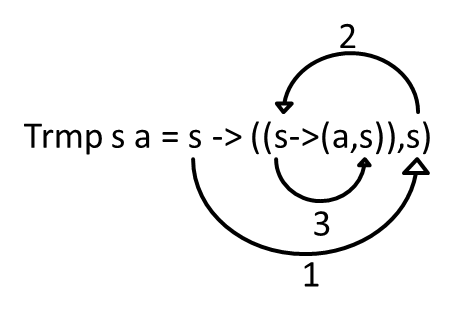
\psfig{file=TrmpDiagram.png,height=5cm}} 
\caption{State flow\label{fig:trampoline_diagram}}
\end{figure}

A trampoline is constructed from the captured values that will have a lifetime at least as long as that of the trampoline and the actual body of the trampoline. The first thing the trampoline constructor does is increment the captured values, and then it binds the execution of the body of the trampoline with decrementing the captured values:

\begin{lstlisting}
trmp :: Reference f a s => f a -> (f a -> Trmp s b) -> Trmp s b
trmp ctxt p = \s -> (\s ->
  let p',s' = p ctxt s
  in p' (snd (decr ctxt s'))), snd (incr ctxt s)
\end{lstlisting}

We have a return function that creates a trampoline. To make this work we assume that our language supports operator overloading, where the most specific overload will be invoked at each binding site:

\begin{lstlisting}
return :: Reference f a s => f a -> Trmp s (f a)
return x = \s->(\s -> x,snd (incr x s)),s
\end{lstlisting}

We can turn a trampoline into a statement with relative ease by unpacking it and executing it twice:

\begin{lstlisting}
(!) :: Trmp s a -> St s a
!p = \s ->
  let p',s' = p s
  in p' s'
\end{lstlisting}

Even more interesting is the fact that we can easily bind values of the state monad with trampolines;  the result will be another trampoline. This kind of binding starts decrementing the bound value y much sooner than the standard binding, since y get decremented before the full execution of k. The idea is that k has a chance to increment y as its ctxt, and right after this has been done k y returns k'. The actual execution of k is thus stored as k', which may contain recursive calls to some caller. Before executing this (possibly time-consuming) code we get our chance to free y in case it were not needed anymore inside k':

\begin{lstlisting}
(>>=) :: Reference f a s => St s (f a) -> (f a -> Trmp s b) -> Trmp s b
p >>= k = \s ->
  let y,s' = p s
  let k',s'' = k y s'
  in k', decr y s''
\end{lstlisting}

Notice that this version of the binding operator is exactly the same as the original binding operator, and since trampolines are state monads then there is no need for the explicit definition.

\subsubsection{Solving the benchmark problem}

We can rewrite the binary tree example above as:

\begin{lstlisting}
bt :: Reference f [Point] s => f [Point] -> Trmp s Tree [Point]
bt pts =
  if size pts < 1000 then trmp pts (\pts -> return mk_leaf pts)
  else
    trmp pts (\pts ->
      do m <- median pts
         trmp (pts,m) (\(pts,m) ->
           do l,r <- split pts m
              trmp (l,r) (\(l,r) -> 
              do tl <- bt l
                 trmp (tl,r) (\(tl,r) ->
                 do tr <- bt r
                    trmp (tl,tr) (\(tl,tr) ->
                      return mk_node (tl,tr))))))
\end{lstlisting}

where we can clearly see that each continuation declares explicitly what it will keep alive (in terms of reference counting). This is a similar style to the well-known world-passing-style of the state monad, but we are also passing around the active scope.

\subsubsection{Syntactic sugar for continuations}

It is very important to notice a detail that threatens the correctness of our system. Continuations may not capture values whose type respects the Reference predicate; continuations may only use those counters that they explicitly captured, otherwise we have no guarantee that the captured counter will still be valid when accessed.
For this reason we introduce a notion of syntactic sugar for expressing our continuations where the captured variables are the free variables of type Reference accessed in the body of the continuation. We tell the compiler to search for these variables with the trmp keyword (not to be confused with the private trmp function seen above).
The translation rule is quite straightforward:

\begin{lstlisting}
	[| trmp x <- m n |] = trmp ctxt (\ctxt -> m >>= fun x -> [| trmp n|])	
	where ctxt = FC(m) $\cup$ FC(n)

	[| trmp return m |] = trmp ctxt (\ctxt -> return m)
	where ctxt = FC(m)
where FC(t) = {x:f a $\in$ FV(t) : $\exists$s . Reference f a s}
\end{lstlisting}

The resulting code is:

\begin{lstlisting}
bt :: Reference f [Point] s => f [Point] -> Trmp s Tree [Point]
bt pts =
  if size pts < 1000 then trmp return mk_leaf pts
  else
    trmp m <- median pts       -- FC = pts
       l,r <- split pts m      -- FC = m,pts
       tl <- bt l              -- FC = l,r
       tr <- bt r              -- FC = r,tl
       return mk_node (tl,tr)  -- FC = tl,tr
\end{lstlisting}

and since we can easily see that:

\begin{lstlisting}
FC(trmp m <- median pts
        l,r <- split pts m 
        tl <- bt l 
        tr <- bt r 
        return mk_node (tl,tr)) = pts
FC(trmp l,r <- split pts m 
        tl <- bt l 
        tr <- bt r 
        return mk_node (tl,tr)) = (pts,m)
FC(trmp tl <- bt l 
        tr <- bt r 
        return mk_node (tl,tr)) = (l,r)
FC(trmp tr <- bt r
        return mk_node (tl,tr)) = (tl,r)
FC(return mk_node (tl,tr)) = (tl,tr)
\end{lstlisting}

then it is clear how the sample with implicit continuations becomes identical to the one with explicit continuations.

 

\section{Parametrized state monad}
\label{sec:parametrized_state_monad}
%----------------------------------------------------------------------------
%  parametrized_state_monad.tex 
%----------------------------------------------------------------------------
We now move to a more powerful definition of the state monad, the parametrized state monad \cite{1_7}. This new version of the monad allows statements to make (static) changes to the state type, rather than just (dynamic) changes to the state value. The parametrized state monad has the following type:

\begin{lstlisting}
type St p q a = p -> (a,q)
\end{lstlisting}

The definition of a counter can now take advantage of the knowledge that all the proxies f a point to the same type of storage (lists, lists of lists, maps, arrays, etc. as seen in Reference implementation), and a value with the storage type must be present in the state whenever we manipulate a proxy:

\begin{lstlisting}
class Reference f a where
  Storage f a :: *
  emptyStorage :: Storage f a
  new :: (s_a ~ Storage f a, Addable s_a s, s_a $\in$ s_a .+ s) => a -> St s (s_a .+ s) (f a)
  incr :: (s_a ~ Storage f a, s_a $\in$ s) => f a -> s -> s
  decr :: (s_a ~ Storage f a, s_a $\in$ s) => f a -> s -> s
  get :: (s_a ~ Storage f a, s_a $\in$ s) => f a -> St s s a
  count :: (s_a ~ Storage f a, s_a $\in$ s) => f a -> St s s Int
\end{lstlisting}

In particular Storage f a is the type function that associates the type of proxies with the type of actual containers. We also define the value of the empty storage with the property emptyStorage. The new function requires that the appropriate storage gets added to the input type of the state; the (idempotent) addition of an element to a heterogeneous list \cite{4_1,4_2} is the .+ operator. The added item must be available in the resulting type, and to ensure this we use the $\in$ predicate. incr and decr both require that the storage is available in the manipulated state (otherwise no incrementing and decrementing could happen because there would be no "slot" to perform the computation in). Similarly we define get and count.
We also define a convenient type-class for types with a default value; this way we can define the default value of a storage as its emptyStorage:

\begin{lstlisting}
class Default x where
  default :: x

instance Reference f a => Default (Storage f a) where
  default = emptyStorage
\end{lstlisting}

 Now we can fill the gaps of the new definition of the Counter type class. A type x can be added to a type s (the result is s .+ x) if it respects the Addable predicate:

\begin{lstlisting}
class Addable x s where
  s .+ x :: *
  add :: s -> s .+ x
\end{lstlisting}

A type x is part of the heterogeneous list s if it respects the $\in$ predicate; this predicate has two instances with respect to the heterogeneous lists constructor (.:):

\begin{lstlisting}
class x $\in$ s where
  lift :: (x -> x) -> (s -> s)

instance x $\in$ x .: s
  lift f = \(x .: s) -> (f x) .: s
instance x $\in$ s => x $\in$ y .: s
  lift f = \(y .: s) -> y .: (lift f s)
\end{lstlisting}

When we wish to add a type x to another type s, we need to check if x$\in$s; if this is the case, then the addition is simply the identity with respect to s (x is already in s). If x?s then the addition returns a heterogeneous list with x as the head and s as the tail, and the value of the head is the default value of x:

\begin{lstlisting}
instance (Default x, x $\in$ s) => Addable x s where
  s .+ x = s
  add = id

instance (Default x) => Addable x s where
  s .+ x = x .: s
  add s = default .: s
\end{lstlisting}

At this point we can define the "regular" binding operator. When binding we need to be able to decrement the bound value of type f a inside the final state, which in our case has type r. For this reason we require that Storage f a$\in$r, so that we will be able to lift the decrementing operation from Storage f a->Storage f a into r->r:

\begin{lstlisting}
(>>=) :: (Reference f a, Storage f a $\in$ r) => St p q (f a) -> (f a -> St q r b) -> St p r b
s >>= k = \p ->
  let x,q = s p
  let y,r = k x q
  in y,lift (decr x) r
\end{lstlisting}

We omit the adaptation of trampolines to the parametrized monad as it is relatively straightforward.

As a side note, it is worth realizing that a big part of the above code, especially the $\in$ predicate, will not work in current incarnations of the Haskell language and will rather give problems that can be solved (albeit in a rather verbose fashion) as seen in the \cite{4_1}. Seen that we have used the above definitions to implement our own custom meta-programming library in F\#, this has not been a problem for us.
 

\section{Related work}
\label{sec:related_work}
%----------------------------------------------------------------------------
%  related_work.tex 
%----------------------------------------------------------------------------

\subsubsection{Region-based memory management}
Tofte and Talpin \cite{8_7} present an inference system for classifying all allocated data of a program into regions and deducing a safe lifetime for each region, which enables provably memory-safe implementations of ML-like languages with-out a garbage collector. Crary et al.'s Capability Calculus \cite{8_6} extends this work by allowing explicit region allocation and deletes, while making sure that all data accesses to a region happen during its lifetime. The commonality of these systems is that only regions are treated linearly; all other objects are allocated within regions and have types akin to guarded types. Regions are not first-class values and cannot be stored in data structures.

\subsubsection{Linear type systems}
Starting with Wadler \cite{8_5}, linear types systems have been used in purely functional languages to enforce single threading on the state of the world or to implement operations like array updating without the cost of a full copy. Linear type systems enable resource management at the granularity of a single object. Every use of an object of linear type consumes the object, leading to a programming style where linear objects are threaded through the computation. Wadler's let! construct, or its variations, can be used to give a temporary nonlinear type to an object of linear type. Walker and Watkins \cite{8_8} study a type system with three kinds of objects: linear, reference counted, and region allocated. The kind of an object is fixed at allocation without a means to change kind. They provide let! only for regions.

\subsubsection{Lighweight static capabilities}
Static capabilities have been implemented by Kiselyov et al. \cite{5_3} in a lightweight fashion in modern functional languages such as OcaML and Haskell. They propose a "style" of programming with three ingredients:
\begin{itemize}
\item A compact kernel of trust that is specific  to the problem domain.
\item Unique names (capabilities) that confer rights and certify properties, so as to extend the trust from the kernel to the rest of the application.
\item Static (type) proxies for dynamic values.
\end{itemize}
The requirements imposed on the host language to implement this style are an expressive core language, higher-rank polymorphism and phantom types. Capabilities are represented as types; safety conditions are stored in types as in dependent-type programming. If a program type-checks, then the type system and the kernel of trust together verify that the safety conditions hold in any run of the program. In most cases, this static assurance costs us no run-time overhead.

\subsubsection{Lightweight Monadic Regions}
Kiselyov et al. \cite{5_1} also build a library that statically ensures the safe use of resources such as file handles. They statically prevent accessing an already closed handle or forgetting to close it. The libraries can be trivially extended to other resources such as database connections and graphic contexts. Their library supports region polymorphism and implicit region subtyping, along with higher-order functions, mutable state, recursion, and run-time exceptions. A program may allocate arbitrarily many resources and dispose of them in any order, not necessarily LIFO. These monadic regions are implemented in Haskell as monad transformers. For contrast, the authors also implement a Haskell library for manual resource management, where deallocation is explicit and safety is assured by a form of linear types. The linear typing is implemented in Haskell with the help of phantom types and a parameterized monad to statically track the type-state of resources.

\subsubsection{Strongly Typed Memory Areas}
Jones et al. \cite{5_4} discuss how to make Haskell suitable for systems programming tasks -including device driver and operating system construction. As a result of some gaps in functionality it often becomes necessary either to code some non-trivial components in more traditional but unsafe languages like C or assembler, or else to adopt aspects of the foreign function interface that compromise on strong typing and type safety. Some of these gaps may be filled by extending a Haskell-like language with facilities for working directly with low-level, memory-based data structures. The authors designed and implemented language features that allow programmers to de?ne strongly typed, high-level views, comparable to programming with algebraic datatypes, on the underlying bitdata structures. A critical detail in making this work is the ability to specify bitlevel layout and representation information precisely and explicitly; this is important because the encodings and representations that are used for bitdata are often determined by third-party speci?cations and standards that must be carefully followed by application programmers and language implementations.
 

\section{Conclusions and future work}
\label{sec:conclusions}
%% Changed by PS, April 4, 2014.

\section{Future work}
\label{sec:future_work}
The Casanova 2 language is capable of implementing usable and quite complex games. The language, while usable, is currently still in development as it misses a few features. In particular, support for multiplayer games is at this moment lacking. We believe that the existing mechanisms for handling time offered by Casanova 2 could be augmented with relatively little effort in order to greatly simplify the hard task of building multiplayer games. This is part of future work, that we are currently engaging in. We are also doing usability studies using students from various disciplines and backgrounds.

The high level view of the game that the Casanova 2 compiler provides can be exploited in order to improve the programmer experience. This means that we could use tools for code analysis (such as abstract interpretation \cite{nielson1999principles} or type system extensions) in order to better understand the game being built, and to help with correctness analysis, performance analysis, or even optimization.


%\subsection{User study}
%We wish to perform an in-depth user study for Casanova 2 to improve usability in the development process. We have already performed a partial (and quite promising) small user study which we will extend and complete.


%We have performed the following test: we gathered a group of students of game programming and a group of students of game design. We gave them a series of Casanova 2 samples, printed on paper. Each student had to guess the functionality of each sample, and sketch a screen-shot. Furthermore, each student also provided some additional feedback on the language.

%The samples were: (\textit{i}) a string of text moved around the screen with the keyboard, (\textit{ii}) a string of text that moves along a predefined path automatically, and (\textit{iii}) an asteroid shooter.

%Eleven (over a total of thirteen) students understood the samples completely, both drawing the screen-shots and explaining the dynamics of the game correctly. Two students were lost on the syntactic differences between Casanova 2 and the more familiar C-like syntax. The direct feedback was mostly centred around a series of common observations, which are reported in Table \ref{students_feedback}. For each observation, the table reports how many times we encountered it.

%\begin{table}[!t]
%% increase table row spacing, adjust to taste
%\renewcommand{\arraystretch}{1.3}
% if using array.sty, it might be a good idea to tweak the value of
% \extrarowheight as needed to properly center the text within the cells

%\caption{Feedback from students}
%\label{students_feedback}
%\centering

%% Some packages, such as MDW tools, offer better commands for making tables
%% than the plain LaTeX2e tabular which is used here.
%\begin{tabular}{|c||c|}
%\hline
%Syntax is unfamiliar at first & 3\\
%\hline
%Syntax is clear & 8\\
%\hline
%Indentation instead of parentheses is a downside & 2\\
%\hline
%List processing with queries is very effective & 1\\
%\hline
%Rules are a good abstraction for games & 2\\
%\hline
%\end{tabular}
%\end{table}

%We also built a significantly bigger sample, which we asked only three students to study. The sample is a checkpoint-based RTS (see Figure \ref{RTS game} for a screenshot). All students correctly identified the game mechanics, and provided some additional feedback. Most of this feedback overlaps with that obtained for the samples, but some new observations emerge. Arguably, some patterns become visible only with larger samples:
%\begin{itemize}
%\item \texttt{wait} and \texttt{when} are very powerful
%\item Multiple rules on the same field are very powerful
%\item Multiple rules on the same field may lead to behaviours that are complex to understand
%\end{itemize}


\section{Conclusions}
\label{sec:conclusions}

Casanova 2, a language specifically designed for building computer games, may offer a solution for the high development costs of games. The goal of Casanova 2 is to reduce the effort and complexities associated with building games. Casanova 2 manages the game world through entities and rules, and offers constructs (wait and yield) to deal with the run-time dynamics. As shown by the benchmarks in Section \ref{sec:evaluation}, we believe that we have taken a significant step towards reaching these goals. In fact, we achieved at the same time very good performance and simplicity, thereby empowering developers with limited resources.  

\bibliographystyle{plain}
\bibliography{references} 
\cite{*}
\nocite{}

\end{document}
